\documentclass[11pt]{scrartcl}
\usepackage[parfill]{parskip}
\usepackage{graphicx}
\usepackage{booktabs}
\usepackage{tabulary}
\usepackage{float}
\usepackage{eurosym}
\usepackage{hyperref}

\graphicspath{{../images/}}

\title{\textbf{Project Management}}
\subtitle{WebKit bug reporting guidelines}
\author{Ricardo Garc\'ia Fern\'andez}
\date{\today}

\begin{document}

\maketitle

\vfill

\begin{flushright}
    \copyright  2013 Ricardo Garc\'ia Fern\'andez - ricardogarfe [at] gmail [dot] com.

    This work is licensed under a Creative Commons 3.0 Unported License.
    To view a copy of this license visit:
 
    \url{http://creativecommons.org/licenses/by/3.0/legalcode}.
\end{flushright}

\begin{figure}[h]
    \begin{flushright}	
        
\includegraphics{by}
        \label{fig:by}
    \end{flushright}
\end{figure}

\newpage

\section{Questions}

\par Analyze the following bug reporting guidelines from the WebKit project:

\url{http://www.webkit.org/quality/bugwriting.html} 

\par Pick up another popular FLOSS project/community with similar guidelines and find similarities and differences. After this, can you briefly summarize which are (in your own opinion) the most relevant guidelines for submitting appropriate bug reports to a FLOSS project. What is the role of automated bug reporting systems in this process?

\section{WebKit guidelines}
\label{sec:webkit-guidelines}

\begin{enumerate}
	\item \textbf{Version}: Select WebKit version: 537.11
	\item \textbf{Component}: Select cause to specific component: CSS, HTML Editing
	\item \textbf{Platform and OS}: Complete OS field (Ubuntu 12.04)
	\item \textbf{Priority}: This field will be set up by Q\&A member, but you have a guide to choose it at \url{http://www.webkit.org/quality/bugpriorities.html}
	\item \textbf{Severity}: the main case is \emph{normal}, but you could choose between \emph{trivial} or \emph{enhancement}. Q\&A member will check this field.
	\item \textbf{URL}: Fill the field with URL that replicates the bug. There is also a guide for this section, Test Case Reduction\footnote{\url{http://www.webkit.org/quality/reduction.html}}.
	\item \textbf{Summary}: \emph{One should be able to tell exactly what a bug is about just by reading the summary}. It's the most important part and has to be well redacted and clear for everyone. Replicate the error, URL, is a REGRESSION bug ? if it's a REGRESSION, which bug points to?
    \item \textbf{Description}: Detailed explanation of the problem. Include only one bug, WebKit version (release, nightly build, etc\ldots), URLs, log messages, backtrace, screenshot for visual bugs. \textbf{Be specific}.
     \item \textbf{Keywords}: Select specific Keywork for tagging the bug. There is a guide for standard Keyword in WebKit Bugzilla\footnote{\url{https://bugs.webkit.org/describekeywords.cgi}}.
     \item \textbf{Depends on}: If the fix for this bug depends on another bug fix, attach bug's number.
     \item \textbf{Blocks}: If this bug blocks another bug, select related bug.
\end{enumerate}

% section webkit-guidelines (end)

\section{Spring-ROO bug tracker}
\label{sec:spring-roo-jira}

\par Spring community guide \emph{Get Invloved}\footnote{\url{http://www.springsource.org/get-involved}}, aims us to report issues related to each Spring module in Issue Tracking System (Included Bugs).

\par So I choose Spring-ROO Issues/Bug tracker\footnote{\url{https://jira.springsource.org/browse/ROO}} to compare with WebKit BTS -\emph{Bug Tracking System}-. Spring-ROO uses JIRA\footnote{\url{http://www.atlassian.com/en/software/jira/overview}} instead of Bugzilla\footnote{\url{http://www.bugzilla.org/}} that is used by WebKit.

\par Go to Spring-ROO JIRA web, and create new bug. JIRA shows this popup:

\begin{figure}[htp]
    \begin{flushright}	
        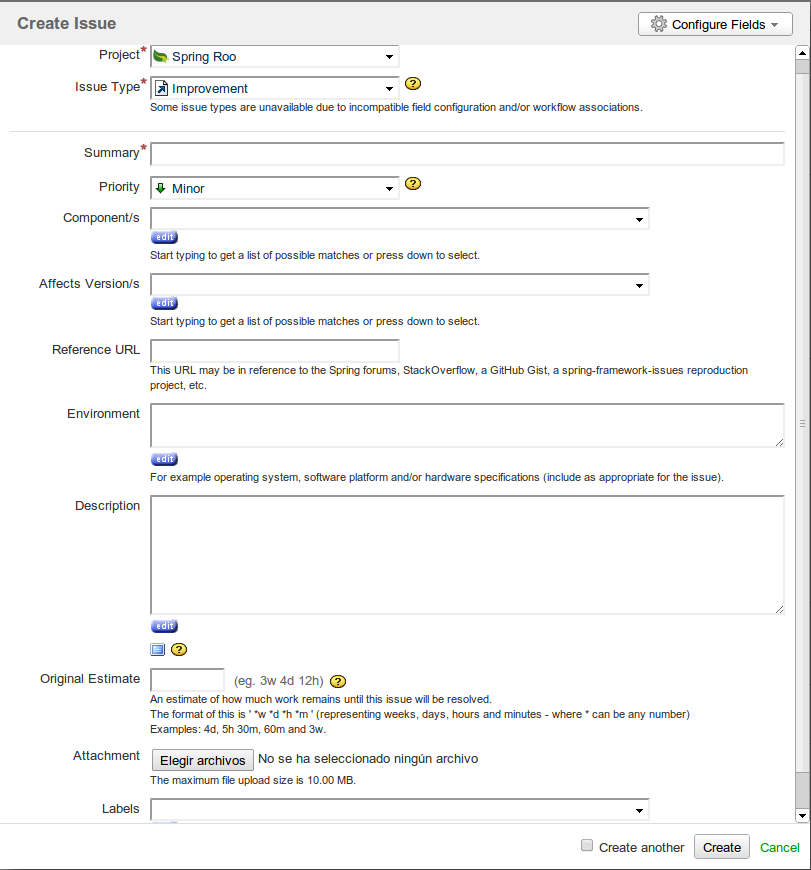
\includegraphics[width=0.9\textwidth]{spring-roo-jira-bug-tracker.png}
        \label{fig:spring-roo-jira}
    \end{flushright}
\end{figure}

\par After open it, we can go to Bug Guideline at \url{https://jira.springsource.org/secure/ShowConstantsHelp.jspa?decorator=popup#IssueTypes} and read Spring bug reporting statements:

\begin{enumerate}
	\item \emph{the issue type}: show issues type list to choose.
	\item \emph{a summary}: Brief summary of the bug.
	\item \emph{a description of the issue}: More complete description about the bug you are reporting. \textbf{Be clear and specific}. How to replicate the Issue.
	\item \emph{the project which the issue belongs to}: In this case Spring-ROO.
	\item \emph{components within a project which are associated with this issue}: Which component/s in project is/are affected by this bug.
	\item \emph{versions of the project which are affected by this issue}: Spring- ROO Version to replicate the bug.
	\item \emph{versions of the project which will resolve the issue}: This is for Spring-ROO team.
	\item \emph{the environment in which it occurs}: Environment, OS, platform, related libraries,\ldots
	\item \emph{URL}: Forum url for comments, reproductions, project, etc.
	\item \emph{Original Estimate}: Estimate of how much work until its resolved.
	\item \emph{Attachments}: Files to help to resolve the issue.
	\item \emph{Labels}: Tags for the issue. This helps to find related issues and help.
	\item \emph{Issues links}: Related issues that could depend or block this work.
	\item \emph{a priority for being fixed}: You can set the priority, but will be tested by developers to give a more realistic value.
	\item \emph{an assigned developer to work on the task}: This is for Developers Team, after read the Bug/Issue.
	\item \emph{a reporter} - the user who entered the issue into the system: Filled automatically with your Spring-ROO JIRA user data.
	\item \emph{the current status of the issue}: Status changed by Developers.
	\item \emph{a full history log of all field changes that have occurred}: Log history for each issue.
	\item \emph{a comment trail added by users}: Log history comments.
	\item \emph{if the issue is resolved - the resolution}: Final result explained by developer.
\end{enumerate}

% section spring-roo-jira (end)

\section{Similarities and Differences}
\label{sec:similarities-and-differences}

\par We can see the similarities outweigh the differences.

\par Bug-Trackers Both make great stress upon definition versions of their projects. The environment where the bug has been found and as you can reply, accompanied by a clear and specific description of how we got the bug. The section which specifies the component where the bug is found and the tag that you assign.
Also if there is a related bug that may affect the new bug.

\par One similarity to note is the reference for regarding the error logs. The logs are written by the application, so they are clearer and there is not a different interpretation by each person. It is a way to avoid the 'human error' and certify the error.

\par Above all we can get the idea that the most important thing is to make a clear description of the bug is and how to replicate it.

\par More technical data developers are responsible, such as the priority, the resolution time and severity.

\par Furthermore, the few differences that can be found in the different \emph{BTS} are related to the collection of information. By \emph{Spring-ROO}, emphasis is on linking the Bug with other sources of data, such as for forums, websites to unify the information in one source and not waste any source.

% section similarities-and-differences (end)
\section{Most relevant}
\label{sec:most-relevant}

\par In my opinion, most relevant guidelines in a \emph{BTS} are in common with \emph{WebKit} and \emph{Spring-ROO}. 

\begin{itemize}
	\item Write a \textbf{clear and specific summary and description} about the bug.
	\item Information about the environment and version affected.
	\item Describe how to replicate the bug, step by step and which tools you used (version, etc\ldots).
	\item Log information, traces.
\end{itemize}

% section most-relevant (end)
\section{Automated Bug Reporting Systems}
\label{sec:auto-brs}

\par The BRS attempt, through a basic standard of information, create a bug, without disturbing the user. That is, bugs are sometimes lost by the mere fact that a person has to attach the error that happened in the corresponding BTS. This person may not know what a BTS, not feel like registering at another site, the error does not stop you keep doing your job, you had a bad experience in other BTS, invest time in it, does not know how to report bugs, anything related to the 'human behaviour' of each of us.

\par Therefore, the automatic transmission bugs, try to gather information when there is a bug in the project automatically, environment, version, related projects, record logs, user, through a friendly interface that the person has the option sending the error, ie, know what you are doing without having to invest almost no time. This will collect more bugs and you can get more information and different statistics of bugs replicated in different environments.

\par And if the person wants to track closer you are given the option to get involved in solving the bug, but that has to look for information. For thus user collaboration more accurate and show their level of involvement. So bugs will be more accurate and better drafted.

% section auto-brs (end)
\end{document}
